\section{The Decomposition Algorithms}
\label{sec:algo}

This section of the manual describes, hopefully without too much techinical detail, the curve and surface decomposition algorithms.  The main academic paper on this is \cite{besana2013cell}, while the paper on Bertini\_real implementing it is \cite{BrN15}.  Two additional extended abstracts discussing it are \cite{Brake2014, On14}.

We invite you to play with the software and visualization routines, to experience these algorithms first-hand.  Dani in particular thinks of these algorithms as implementations of the implicit function theorem.  Enjoy!


\subsection{Decomposing curves}
\label{sec:algo_curve}



Decomposing an algebraic curve numerically can be summarized easily in six steps:
%
\begin{enumerate}[noitemsep]
\item Compute critical points
\item Intersect with bounding object
\item Slice at projection interval midpoints
\item Connect the dots
\item Merge [optional]
\item Sample [optional]
\end{enumerate}

A curve is decomposed with respect to projection onto a (randomly chosen) real linear projection, $\pi_0(x)$.


What does it mean to decompose a curve?  To turn compute a set of {\em edges} that describe the curve.  An edge is a 1-dimensional object, having two points as boundary, and a general point in the middle, together with a homotopy which can be used to track the midpoints between the boundary points.  Phew.  See Figure~\ref{fig:edge}.




\begin{figure}[H]
\begin{center}
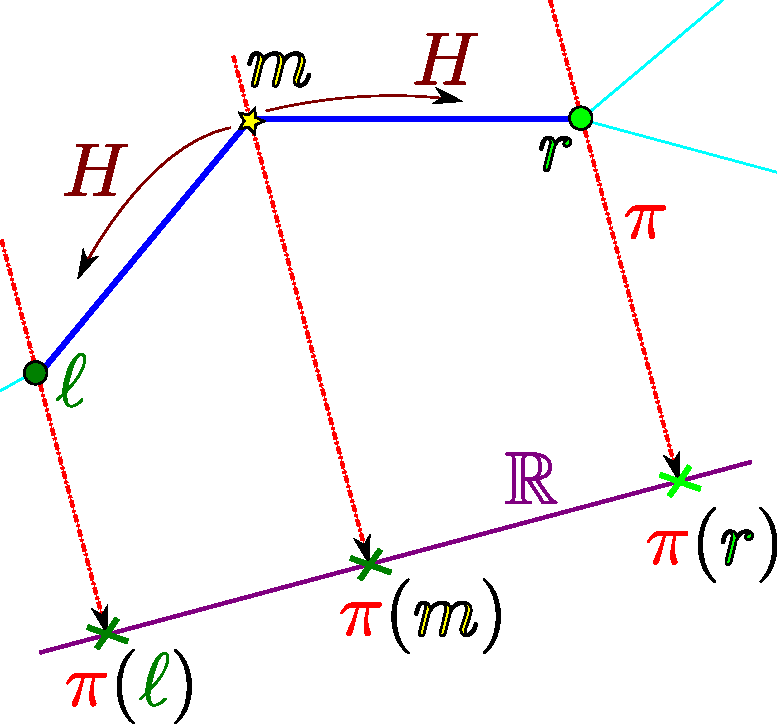
\includegraphics[width = 2in]{edge}
\caption{An edge, a 1-cell, as a component of a curve decomposition.}
\label{fig:edge}
\end{center}
\end{figure}


\subsubsection{Critical points}

Critical points of a curve satisfy the following system:
\begin{equation}
\begin{bmatrix}
f(x) \\
\textnormal{det} \begin{pmatrix} Jf(x) \\ J\pi_0 \end{pmatrix}
\end{bmatrix}  = 0. \label{eqn:curve_critpts}
\end{equation}
These points include singular points (trivially, and independently of projection).  This is solved by a 2-homogeneous regeneration procedure.


\subsubsection{Intersect with bounding object}

To capture the behaviour of the curve as it goes to $\infty$, we intersect the curve with a bounding object, and ignore all outside points.  In Bertini\_real, we use a sphere centered at the centroid of the critical points, with radius 3 times the distance to the furthest critical point.  The user can choose their own sphere of interest.


\subsubsection{Slice}


Let the set of critical points just computed be $\chi$.  Then, take $\pi_0(\chi)$, the set of critical projection values.  We slice at midpoints of projection intervals defined by this set.  This computes the set of midpoints for (unmerged) edges computed by the next step.


\subsubsection{Connect the dots}
\label{sec:connect_curve}


Connecting the dots for a curve simply means to track each midpoint to the left and right bounding critical projection values, and see what critical points match.  This forms an edge.  The homotopy 
\begin{equation}
(1-t)
\begin{bmatrix}
f(x) \\
\pi_0(x) - p_{c_j}
\end{bmatrix}
+t
\begin{bmatrix}
f(x) \\
\pi_0(x) - p_{m_i}
\end{bmatrix} = 0\label{eqn:projvalmove}
\end{equation}
is used.

Some midpoints may track to points in critical fibers which have not yet been previously computed.  In software, these are classified as {\em semicritical}.

\subsubsection{Merge [optional]}

Merging edges combines two edges which meet at a non-critical point.  These points occur when tracking midpoints toward critical projection values yields a new point, one in the fiber of a true critical point.  A simpler curve decomposition can be obtained by merging such edges.  There are times when merging is great (most of the time) and times when merging is not the right thing to do (some points in the surface decomposition algorithm).

Merging can be disabled when decomposing a curve in Bertini\_real with the {\tt -nomerge} flag.


\subsubsection{Sample [optional]}
Suffice it to say for now that a midpoint is tracked using \eqref{eqn:projvalmove} within the bounds of its edge, producing additional points on the edge.  
This section is described in much greater detail in Section~\ref{sec:sampler_curve}.   



















\subsection{Decomposing surfaces}
\label{sec:algo_surface}


Decomposing an algebraic surface numerically is similar to that of a curve, and can also be summarized in about six steps:
%
\begin{enumerate}[noitemsep]
\item Compute critical curves
\item Intersect with bounding object
\item Slice at projection interval midpoints.  The slices are curve decompositions
\item Connect the dots to form faces
\item Merge [optional]
\item Sample [optional]
\end{enumerate}


To decompose a surface is to compute a set of {\em faces}.  A face is a 2-cell, containing a set of bounding edges, and a general point in the middle, which can be tracked using a homotopy, staying within the boundary.  See Figure~\ref{fig:face}

\begin{figure}[H]
\begin{center}
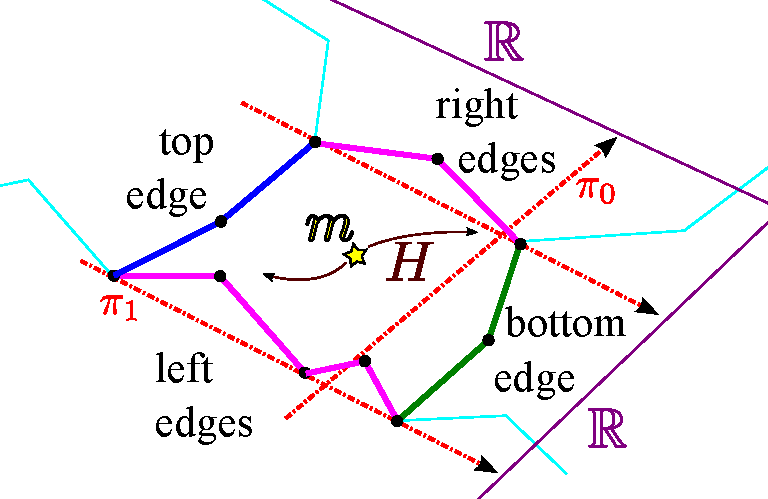
\includegraphics[width = 2in]{face}
\caption{A face, a 2-cell, as a component of a surface decomposition.  Its boundary consists of edges from curve decompositions.}
\label{fig:face}
\end{center}
\end{figure}

A surface is decomposed with respect to projection onto a pair of (randomly chosen) real linear projections, $\pi_0(x)$ and $\pi_1(x)$, together which may be referred to as $\pi(x)$.

\begin{figure}[H]
\begin{center}
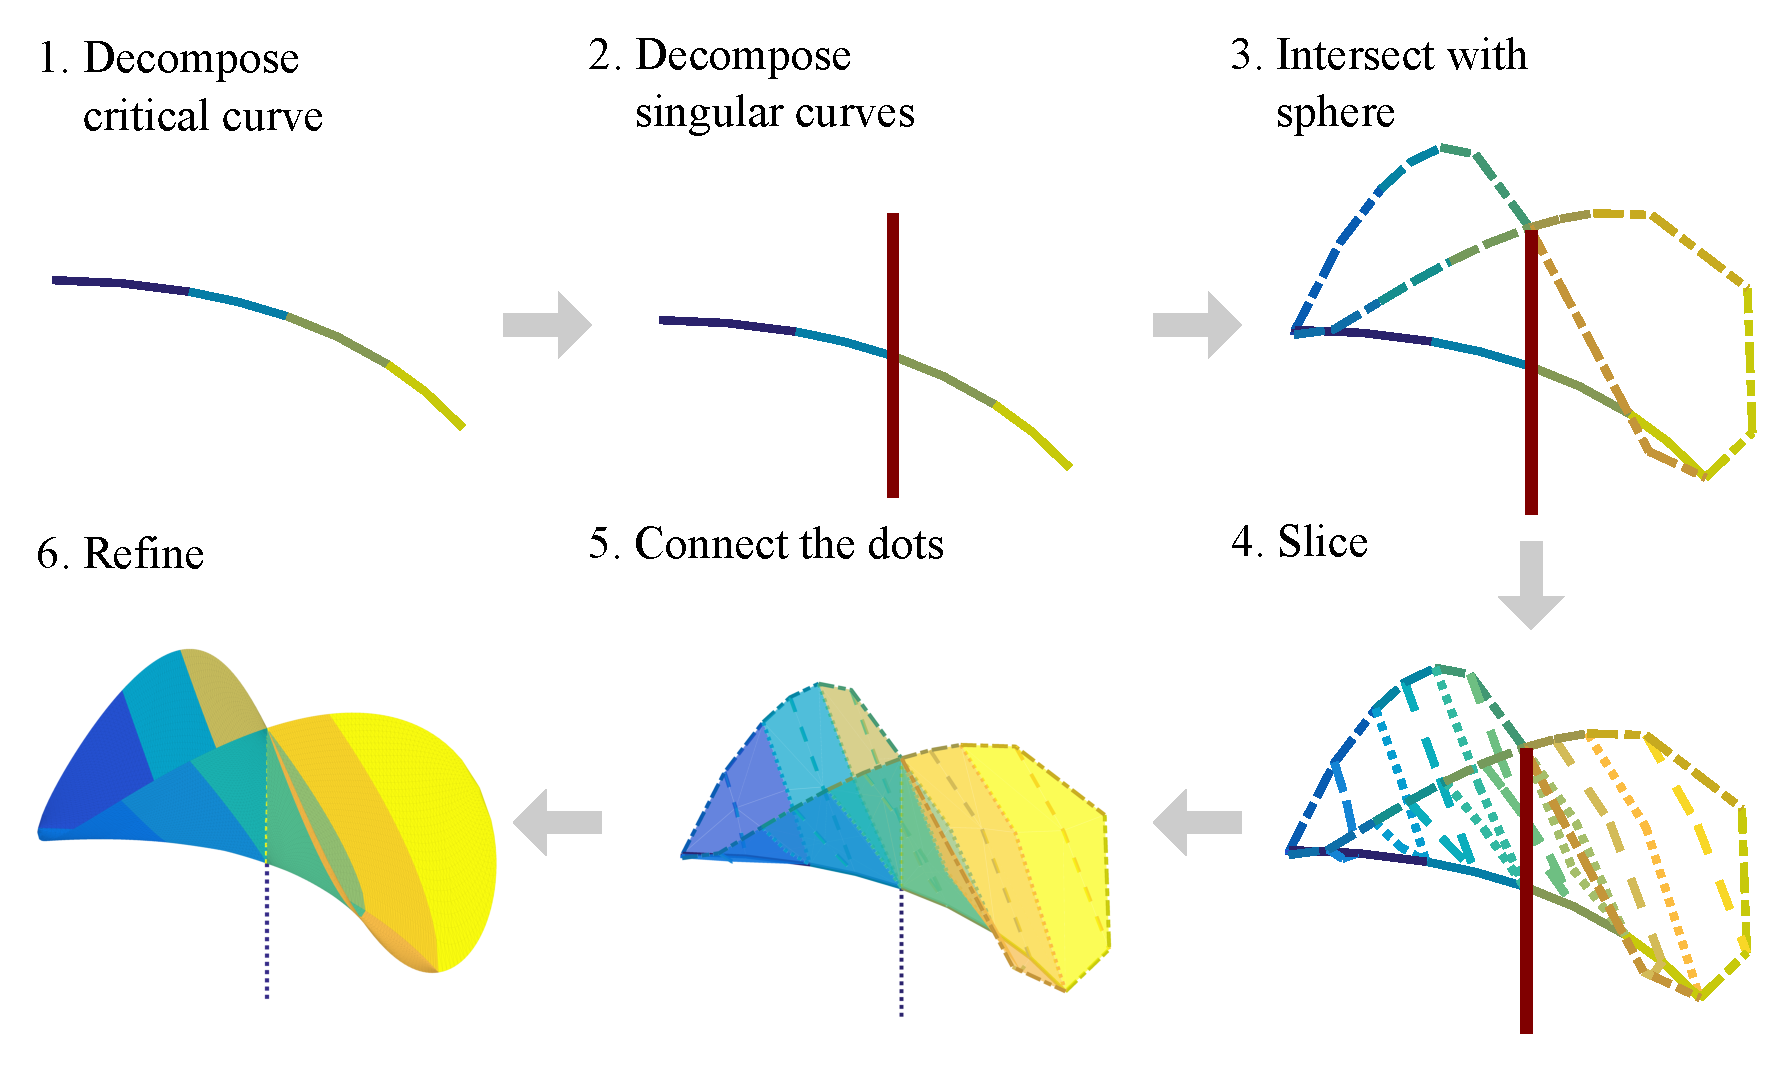
\includegraphics[width = 5in]{surface_method}
\caption{Numerical cellular decomposition of the Whitney Umbrella using Bertini\_real.}
\label{fig:decomposing_surface}
\end{center}
\end{figure}






\subsubsection{Critical curves}

Critical curves can be separated into two categories.  First, those which are an artifact of the projection being used to decompose.  Second, those which appear regardless of the projection.  In this manual and software, we refer to the former simply as the {\em non-singular critical curve} or simply {\em critical curve}, and the second as {\em singular curves}, although they both are formally part of the critical curve (and so is the bounding curve).


\paragraph{Nonsingular critical curve}

The non-singular critical curve satisfies this system, nonsingularly:
\begin{equation}\label{eqn:crit_curve}
    F(x) = \begin{bmatrix}
f(x) \\
\det \begin{pmatrix}
    Jf(x) \\
    J\pi_0 \\
    J\pi_1
            \end{pmatrix} \\
\end{bmatrix} = 0.
\end{equation}
In current implementation using Bertini1 as the homotopy engine, we use a symbolic engine to compute a new text Bertini input file.  There are several options for the symengine, described in Section~\ref{sec:running_br}.  A curve decomposition is run on this curve.  But first, we have to have {\em \bf all} of the critical points of all critical curves, including non-singular, singular, and bounding.


\paragraph{Singular curves}

Not every surface has singular curves, but many do.  Perhaps the easiest to see at first is the Whitney Umbrella.
\begin{equation}
f = x^2 - y^2 z = 0
\end{equation}
This equation describes a degree 3 surface.  The $z$-axis is singular.  Observe the Jacobian:
\begin{equation}
Jf = \begin{bmatrix}
2x & -2yz & -y^2
\end{bmatrix}
\end{equation}
On the $z$-axis, $x = y = 0$.  So, $Jf$ is singular.  Hence the determinant in \eqref{eqn:crit_curve} is $0$, which means the critical curve system is in some sense trivially satisfied.  What is needed here is to {\em deflate} the system.  This is accomplished in current implementation using {\em isosingular deflation} \cite{hauenstein2013isosingular}.  Basically, sub-determinants of the system are recursively added until the rank of the Jacobian stabilizes, where this rank is computed using a witness point for the component being deflated.

The singular curves are decomposed using the curve algorithm, after obtaining {\em all} critical points of {\em all} critical-like curves.

\subsubsection{Bounding curve}

To capture the behaviour of surfaces which are not closed or bounded, we intersect the surface with a bounding object.  The implemented type in Bertini\_real is sphere.  Initially, we had implemented a bounding box, and it was neat, but for higher dimensions, it meant doing more and more curve decompositions, with each of the $2N$ planes.  It got messy.  So, surfaces are used.  They are easier, because the entire bounding curve satisfies a single system, which is merely the original system supplemented with a single degree 2 equation -- that of the sphere.  It eases not only implementation but also runtime.

We compute the sphere automatically, after having computed the critical points of the critical and singular curves (but before decomposing them, for algorithmic reasons).  The sphere is centered at the centoid of all critical points, and its radius is arbitrarily chosen to be 3 times the distance from the center to the furthest critical point.  The user may also supply their own sphere of interest (See Section~\ref{sec:running_br}).




\subsubsection{Slice}


Having decomposed all formal parts of the critical curve, we slice the surface.  Where?  

Consider all critical points of all thus-far computed curves.  Call this set $\chi$.  Then we project onto the first projection coordinate, computing $\pi_0(\chi)$.  This set of values produces the critical slices.  Taking midpoints of all intervals defined by $\pi_0(\chi)$ defines the mid slices.  Each of these slices is computed using a regular curve decomposition.





\subsubsection{Connect the dots}
\label{sec:connect_surface}

This is a fun piece of the puzzle.  In this part of the algorithm, midpoints of edges of midslices are connected to midpoints of edges of critslices.  We track the mid-midpoints using a very special homotopy, the {\em midtrack} homotopy:
\begin{equation}
\begin{bmatrix}
f(x) \\
\pi_0(x) - [(1-u) \pi_{0}(c_i) + u \pi_{0}(c_{i+1})] \\
f_{\textnormal{bottom}}(y) \\
\pi_0(y) - [(1-u) \pi_{0}(c_i) + u \pi_{0}(c_{i+1})] \\
f_{\textnormal{top}}(z) \\
\pi_0(z) - [(1-u) \pi_{0}(c_i) + u \pi_{0}(c_{i+1})] \\
\pi_1(x) - [(1-v)\pi_1(y) + v \pi_1(z)]
\end{bmatrix} = 0. \label{eqn:midtrack}
\end{equation}
%
The homotopy is somewhat hidden in (\ref{eqn:midtrack}) -- as written the $t$-dependence is implicit.  To track the homotopy, we use:
\begin{equation}
\begin{bmatrix}
u \\ v \end{bmatrix}
=
\begin{bmatrix}
(1-t) \,u_{\textnormal{target}} + t \, u_{\textnormal{start}} \\
(1-t) \, v_{\textnormal{target}} + t \, v_{\textnormal{start}}
\end{bmatrix}.
\end{equation}
The values of $u$ and $v$ lie in the unit square, and we must only track inside this square.  The purpose of this homotopy is to ensure that the midpoint never crosses an edge of the critical curve, which bounds the in-construction face to the top and bottom.  That is, if we just did a straight-line homotopy in $\pi_i$ coordinates, we would likely cross this critical boundary, and all bets would be off.  Paths would cross, real points would become complex, and the decomposition would not work.  Hence, this homotopy.  It's used during sampling, too.

Anywho, the midpoints are connected to midpoints.  The midpoints of midslice edges become midpoints of faces in the cell decomposition.  Critslice edges bound the face to the left and right ($\pi_0$), while critcurve edges bound to the top and bottom ($\pi_1$).  There may be any number of left and right edges bounding a face, but exactly one top and bottom edge.    


\subsubsection{Merge [optional]}

The algorithm for merging faces does not yet appear in the literature, though it has been described verbally by Charles Wampler.  Let's write it!  Should be a short paper, probably targeting a conference proceedings.  Contact Dani Brake to co-author it with them.


\subsubsection{Sample [optional]}
This section is described in much greater detail in Section~\ref{sec:sampler_surface}.  For now, suffice it to say that \eqref{eqn:midtrack} is used to track around the midpoint of each face, producing additional points on the face, and that a proper triangulation is maintained.  There are choices about how to sample.  One might think this a trivial problem.  Indeed, in three dimensions, there are many many algorithms for adaptively and optimally triangulating surfaces.  However, in higher dimensions the normal vector doesn't exist, and cross-products cannot be taken, so much of the machinery from 3d breaks.  Bummer.  Go check out the section on {\tt sampler} for more.

